\documentclass[11pt]{article}
\usepackage{amsmath, amssymb}
\usepackage{geometry}
\geometry{margin=1in}
\usepackage{fancyhdr}
\usepackage{lastpage}
\usepackage{parskip} % Better paragraph spacing
\usepackage{titlesec} % Better section formatting
\usepackage{graphicx}
\usepackage{float}
\usepackage[most]{tcolorbox}
\usepackage{lmodern}
\usepackage{caption}
\usepackage{hyperref}

% Define commands for reusable content
\newcommand{\coursename}{COM-402 Advanced Networks}
\newcommand{\lecturenum}{07}
\newcommand{\lecturedate}{\today}
\newcommand{\professor}{Pavlos Nikoupoulos}

\hypersetup{colorlinks=true,linkcolor=blue,urlcolor=blue}

% Configure section spacing
\titlespacing*{\section}{0pt}{2ex plus 1ex minus .2ex}{1.5ex plus .2ex}
% Header / Footer
\pagestyle{fancy}
\fancyhf{}
\fancyhead[L]{\coursename}
\fancyhead[R]{Lecture \lecturenum}
\fancyfoot[L]{EPFL - Computer Science}
\fancyfoot[C]{Author: Jonathan Dutoit}
\fancyfoot[R]{Page \thepage\ of \pageref{LastPage}}

\begin{document}

\begin{center}
  {\large EPFL - Computer Science} \\[0.5em]
  {\Large \textbf{\coursename}} \\[0.5em]
  {\large Lecture \lecturenum\ --- \lecturedate} \\[0.5em]
  {\large Author: Jonathan Dutoit} \\[0.5em]
  {\large Professor: \professor} \\[0.5em]
\end{center}

\vspace{1cm}

\begin{center}
  {\LARGE \textbf{Transporter Layer Continued}}
\end{center}

% Quick centered image
\begin{figure}[H]
    \centering
    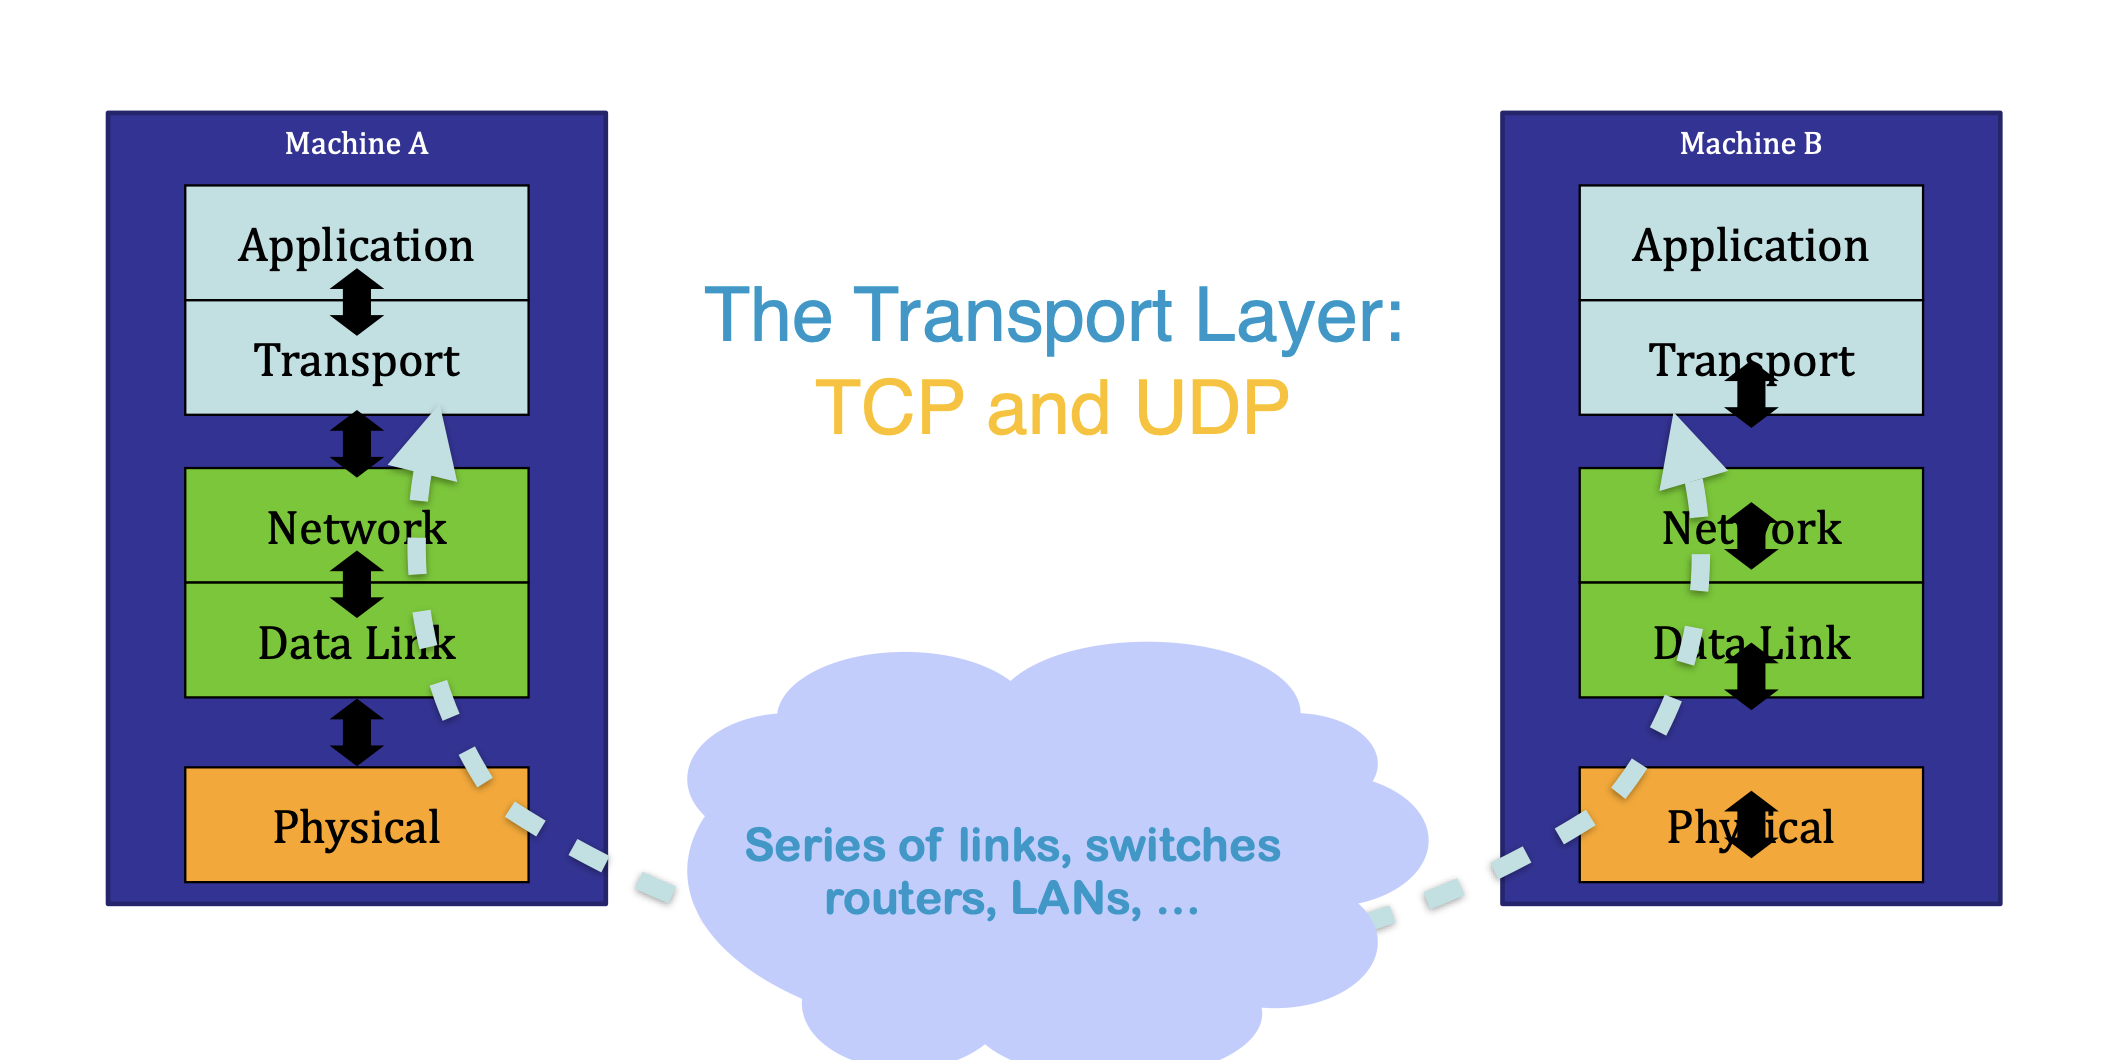
\includegraphics[width=0.65\textwidth]{images/transport-layer}
    \label{fig:LABEL}
\end{figure}
\vspace{1cm}

\begin{tcolorbox}[
  colback=gray!15,     % background color
  colframe=black!50,    % border color
  boxrule=1pt,       % border thickness
  arc=3mm,             % rounded corners
  left=4mm, right=4mm, top=2mm, bottom=2mm % padding
]
\textbf{Window size = 4'000 bytes, one packet = 1'000 bytes. At time $t_0$, the usable part of the sliding window is 4000, and there is a lot of data in the socket to be sent. So, the sender sends 4 segments. At time  $t_1$, sender...}

% Quick centered image
\begin{figure}[H]
    \centering
    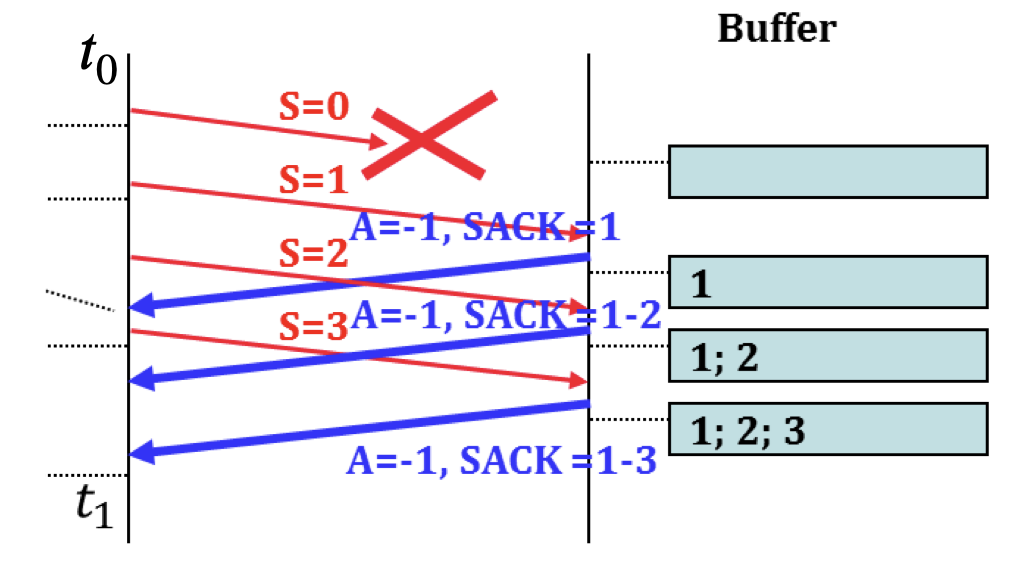
\includegraphics[width=0.4\textwidth]{images/sliding-window-question}
    \label{fig:LABEL}
\end{figure}
\vspace{0.2cm}

A. Can send segment S=4\\
B. Cannot send segment S=4 \\
C. It depends on whether data was consumed by application \\
D. I do not know \\

\textbf{Answer:} B. \\ 
Packet 4 it outside the window [0:3] and cannot be sent. It has to wait until the loss of packet 0 is repaired, which happens at time $t_2$
\end{tcolorbox}
Question follow-up conclusions:
\begin{itemize}
	\item Sender needs a \textcolor{blue}{\textit{retransmission buffer}} to hold unack'ed data; its size is equal to the window size. 
	\item Segments are removed from the resequencing/receive buffer when they are finally put in order and application reads them. 
\end{itemize}

\subsection*{A fixed-size (static) window cannot prevent receive-buffer \textcolor{red}{\textit{overflows}}}
\begin{minipage}{0.6\textwidth}
\begin{itemize}
	\item Sliding window limits the amount of unack'ed/out-of-order data, \\
	\item but in-order data remains in buffer, until applcation reads \\
	\item \textit{\textcolor{blue}{Slowly reading}} receiver app may still trigger buffer overflows
\end{itemize}

\end{minipage}
\hfill
\begin{minipage}{0.4\textwidth}
\centering
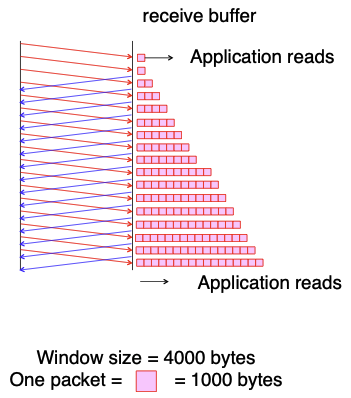
\includegraphics[width=\linewidth]{images/buffer-overflow}
\end{minipage}

\subsection*{Flow control: an \textit{\textcolor{red}{adaptive}} sliding window}
\begin{itemize}
	\item \textcolor{red}{What?} adapt the window size to \textit{\textcolor{blue}{advertisements}} form the other end: 
	\begin{enumerate}
		\item receiver advertizes a window size = available buffer size
			\begin{itemize}
				\item if no space in buffer, advertized window = 0
			\end{itemize}
		\item sender adapts its sliding window to the advertized value
	\end{enumerate}
	\item $\rightarrow$ Flow control adapts source's sending rate to the receiver's \textcolor{red}{\textit{consuming speed}} 
	\item $\neq$ \textbf{Congestion Control}, which adapts source's sending rate to \textbf{\textit{network conditions}}
\end{itemize}

% Quick centered image
\begin{figure}[H]
    \centering
    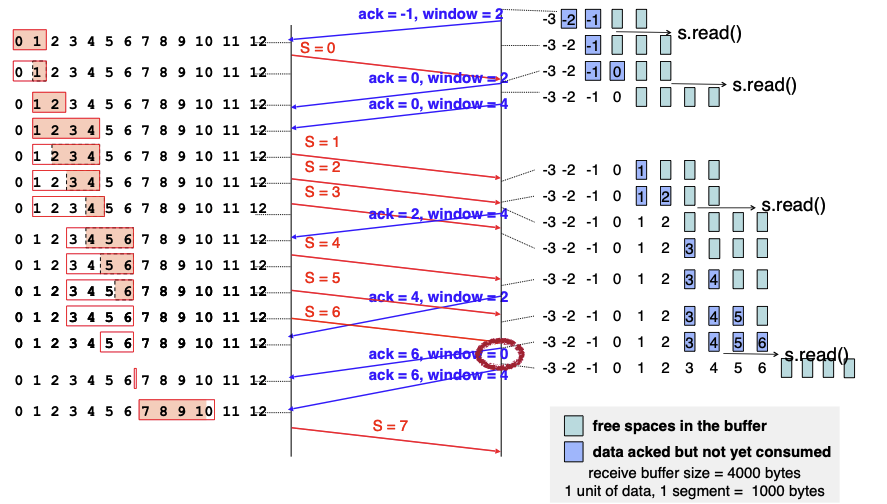
\includegraphics[width=1\textwidth]{images/adaptative-window}
    \label{fig:LABEL}
\end{figure}

\textbf{Note:} the sender can send from time to time a new segments just to re-trigger an acknowledgement from the receiver's side in case of \textbf{the window advertizement packets got lost}. 

\section*{TCP Basic Operation (Recap)}

% Quick centered image
\begin{figure}[H]
    \centering
    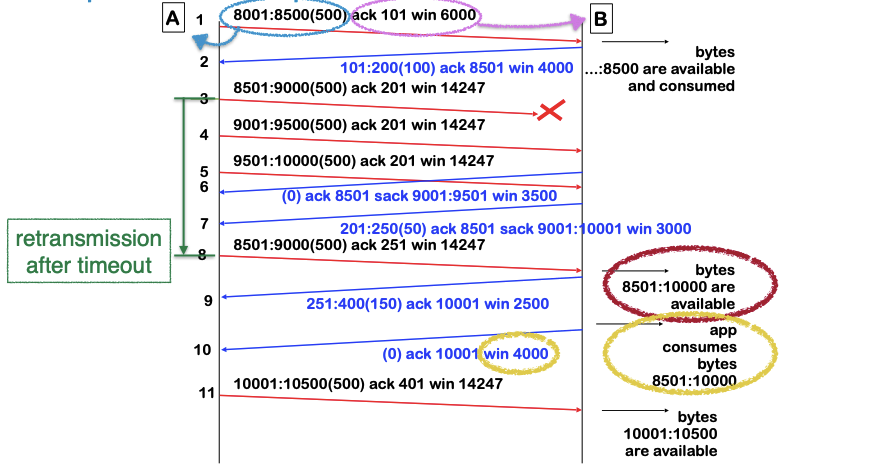
\includegraphics[width=1\textwidth]{images/tcp-basic-operation}
    \label{fig:LABEL}
\end{figure}

\begin{tcolorbox}[
  colback=gray!15,     % background color
  colframe=black!50,    % border color
  boxrule=1pt,       % border thickness
  arc=3mm,             % rounded corners
  left=4mm, right=4mm, top=2mm, bottom=2mm % padding
]
\textbf{If there's no loss or reordering, an on a link with capacity \textit{c} bytes/second, the min window size require for sending at the maximum capacity is...}

\vspace{0.3cm}
A. $W_{min} = RTT \times c$ \\
B. $W_{min} = \frac{c}{RTT}$ \\
C. $W_{min} = \frac{RTT}{C}$ \\
D. None of the above \\
E. I do not know \\

\textbf{Answer}: A. \\
If the window size is large enough, the window is never fully used and the sender can send at rate c. This case occurs when the total amount of data in flight, $c \times RTT$, is not larger than \textit{\textbf{W}}, 
i.e. when $W \geq c \times RTT$ (i.e. window bandwidth-delay product) 
\end{tcolorbox}


\textbf{Note:} A side effect of the streaming service is \textit{\textcolor{blue}{head of the line blocking}} $\rightarrow$ if a packet is lost, all data following this packet cannot read by application, until loss is repaired. 
\begin{tcolorbox}[
  colback=gray!15,     % background color
  colframe=black!50,    % border color
  boxrule=1pt,       % border thickness
  arc=3mm,             % rounded corners
  left=4mm, right=4mm, top=2mm, bottom=2mm % padding
]
\textbf{For which types of apps may TCP's streaming service be an issue (multiple selection is possible)}

\vspace{0.3cm}

A. An app using http/1, where we have several TCP connections, one per object \\
B. An app using http/2, where we have a single TCP connection per webpage \\
C. A real-time sensor-data streaming application that sends a new measurement every msec \\
D. None \\ 
E. I do not know \\

\textbf{Answer:} B and C. \\
Head-of-line blocking may reduce the quality of user's experience in both cases. In the context of HTTP/2 with a single connection: the entire page download will be delayed if a packet is lost in the transfer of one object of the page. 
\end{tcolorbox}

\section*{MSS and segmentation}

TCP, \textit{\textcolor{red}{not}} the application or IP, chooses how to segment data. Segments should \textit{\textcolor{red}{not}} be fragmented at source. 

The maximum segment size (\textcolor{blue}{MSS}) is
\begin{itemize}
	\item either a \textcolor{blue}{\textit{default}} value e.g.:
		\begin{itemize}
			\item 536 bytes when using IPv4
			\item 1220 bytes when using IPv6
		\end{itemize}
	\item or \textit{\textcolor{blue}{negotiated}} in Options header field during connection setup: hosts set it to the \textit{\textcolor{red}{smallest value}} that both declare.
\end{itemize}

Modern OSs use \textcolor{blue}{TCP Segmentation Offloading} (TSO):
\begin{itemize}
	\item Segmentation is done at the network interface card (NIC) with \textit{\textcolor{blue}{hardware}} assistance
	\item Lower CPU load for TCP
\end{itemize}

\section*{3. TCP Connection Phases}
% Quick centered image
\begin{figure}[H]
    \centering
    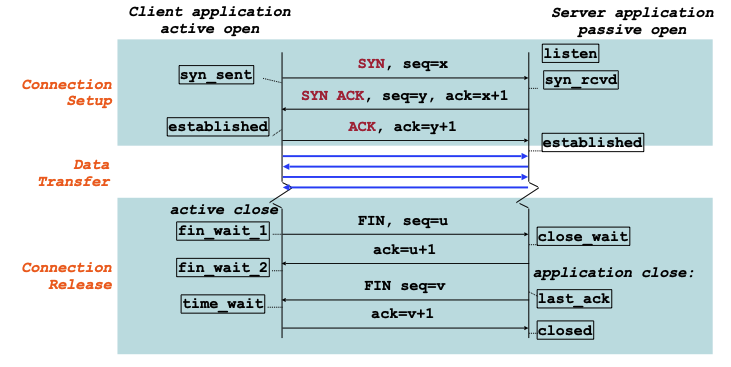
\includegraphics[width=1\textwidth]{images/tcp-connection-phases}
    \label{fig:LABEL}
\end{figure}

% Quick centered image
\begin{figure}[H]
    \centering
    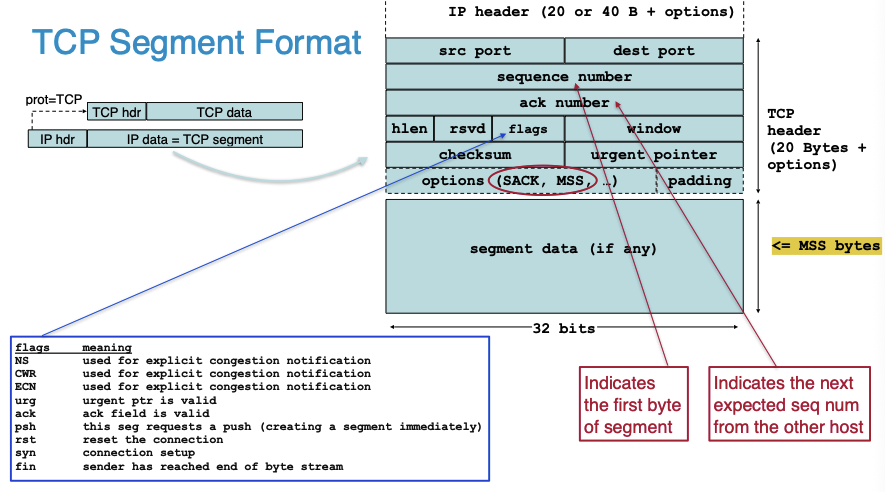
\includegraphics[width=1\textwidth]{images/tcp-segment-format}
    \label{fig:LABEL}
\end{figure}

\section*{TCP Sockets}

\begin{minipage}{0.6\textwidth}
More \textcolor{blue}{\textit{complicated}} than UDP because we need to open/close a connection \\
A TCP connection requires:
\begin{itemize}
	\item one side ("server") to \textit{\textcolor{red}{listen}} and  \\
	\item the other side ("client") to \textit{\textcolor{blue}{connect}} \\
\end{itemize}
\underline{Steps:}\\
\begin{enumerate}
	\item Server enters \textcolor{red}{\textit{syn-rcvd}} state; it stores initial state (client's IP address+port, MSS, etc.), sends SYNACK and waits client's ACK
	\item At client, connection is \textcolor{blue}{\textit{established}}; the socket is used to send/receive data
	\item At server, upon reception of the ACK,  connection is established and a \textcolor{red}{\textit{new socket (conn)}} is created; this will be used to receive/send data
\end{enumerate}

\end{minipage}
\hfill
\begin{minipage}{0.4\textwidth}
\centering
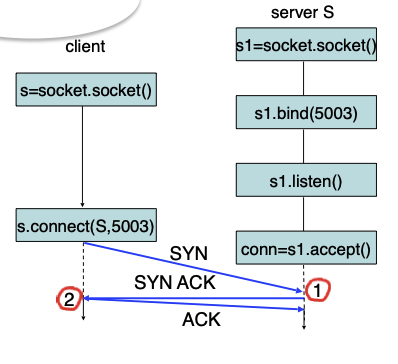
\includegraphics[width=\linewidth]{images/tcp-sockets}
\end{minipage}

Why a new socket?
\begin{itemize}
	\item In practice, multiple clients want to connect to the server
	\item Server creates a new socket per connection
	\item Uses parallel-execution threads
		\begin{itemize}
			\item to listen to incoming connection
			\item to handle several TCP connections
		\end{itemize}
	\item A TCP connection is identified by: \textbf{\{src IP addr, src port, dest IP addr, dest port\}}
\end{itemize}

\section*{How the Operating System view TCP socket?}
% Quick centered image
\begin{figure}[H]
    \centering
    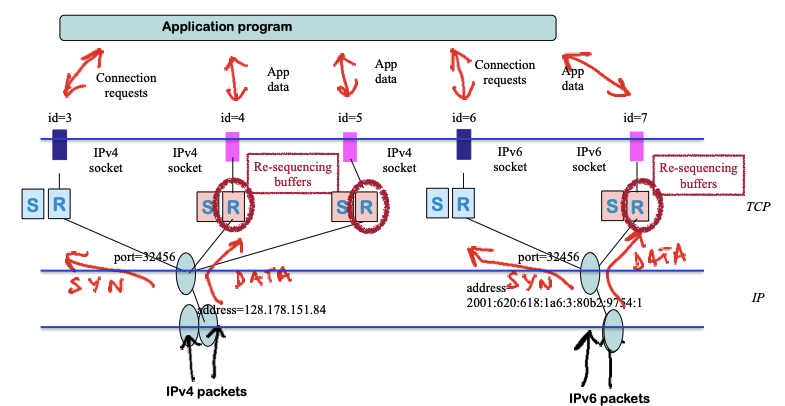
\includegraphics[width=1\textwidth]{images/os-sockets}
    \label{fig:LABEL}
\end{figure}
\section*{Why both TCP and UDP?}

Most applications nowadays use TCP, as this avoids re-inventing error recovery for each app. But some apps may not need TCP-like error recovery (i.e., packet retransmission): 
\begin{itemize}
	\item Voice applications / Sensor data streaming \\
	Q. Why? \\
	\textcolor{blue}{Delay is important for interactive voice, while packet retransmission may introduce too much delay in some cases.} \\
	\textcolor{blue}{Sensor data streaming may send a new packet every few msecs, better to receive latest packet than to repeat a lost one.}
	\item An application that sends just one message, like name resolution (DNS) \\
	Q. Why?
	\textcolor{blue}{TCP sends several packets of overhead before one single useful data message. Such an application is better served by a Stop and Go protocol at the application layer.}
	\item Multicast (TCP does not support multicast IP addresses)
\end{itemize}

\section*{4. More TCP Bells and Whistles}

How to deal with \textbf{corner cases}? Suppose that an application writes few bytes in socket; should TCP create a segment or wait for more bytes? 
\begin{itemize}
	\item \textcolor{blue}{Nagle's algorithm}: send \verb|min{bytes written in one RTT, MSS}|
	\item How to handle silly window-increase advertisements by 1 byte? The idea is similar to Nagle's, we do something simple
\end{itemize}


Window field is 16 bits $\Rightarrow$ ma throughput even for RTT=1msec is $\tilde$ 524Mbps; can we do better?

\begin{itemize}
	\item negotiate a \textcolor{blue}{scaling factor} of the window during connection setup (RFC1323)
\end{itemize}

\begin{tcolorbox}[
  colback=gray!15,     % background color
  colframe=black!50,    % border color
  boxrule=1pt,       % border thickness
  arc=3mm,             % rounded corners
  left=4mm, right=4mm, top=2mm, bottom=2mm % padding
]
\begin{itemize}
	\item How to detect packet loss?
	\item How to avoid SYN flooding (denial of service attack)?
	\item How to avoid the delay of the 3-way handshake?
\end{itemize}

\end{tcolorbox}
\section*{How to detect packet loss?}

Packet loss in TCP is detect via \textcolor{red}{times} and \textcolor{red}{duplicates} ACKs.

The main timers are called \textcolor{blue}{retransmission timeouts (RTO)}, it's set for every packet transmission and when a timer expires (= \textcolor{red}{timeout}), this is interpreted as \textcolor{red}{severe loss} in the channel. Thus, all timers are reset and all un-acknowledged data is marked as needing retransmission

A \textcolor{blue}{duplicate ACK} = a TCP segment where the cumulative ACK value repeats a previously received ACK value. This is interpreted as \textcolor{red}{not-so-severe loss} in the channel. 

\textcolor{blue}{Timers use an estimate of round trip time (RTT)}

\textcolor{red}{Why?} RTO timer must be set to a value $\geq$ RTT, but not too much

 \textcolor{red}{What?} RTT estimation gives an upper bound on the round trip time, used to set the RTO

 \textcolor{red}{How?} it uses a weird formula. RTO increases when there is variability in the RTT. RTO may be significantly larger until it converges back after a sharp discontinuity. 

\begin{tcolorbox}[
  colback=gray!15,     % background color
  colframe=black!50,    % border color
  boxrule=1pt,       % border thickness
  arc=3mm,             % rounded corners
  left=4mm, right=4mm, top=2mm, bottom=2mm % padding
]
Idea: "Instead of waiting for a timeout, TCP can determine that a packet is lost just after a \textit{\textcolor{red}{single}} duplicate ACK is received with a SACK field, and it can quickly retransmit." \\
Is it a good idea?

% Quick centered image
\begin{figure}[H]
    \centering
    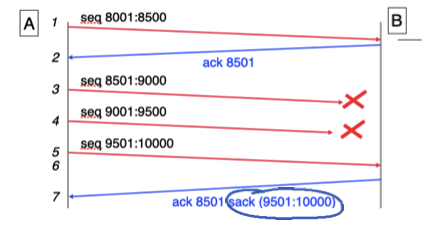
\includegraphics[width=0.55\textwidth]{images/tcp-question}
    \label{fig:LABEL}
\end{figure}
\vspace{0.3cm}

A. Yes because it is likely that there is some missing data \\
B. No as it may cause superfluous retransmissions (some data could simply be late -- out of order) \\
C. NO because an ACK could be lost \\
D. I do not know \\

\textbf{Answer}: There is no “good” answer. \\
Both A and B can be argued. This is why “Fast Retransmit” was invented.
\end{tcolorbox}

\section*{Fast Retransmit}

Principle: when \textit{\textbf{n}} duplicate ACKs are received, declare a loss
\begin{itemize}
	\item \textbf{\textit{n} = TcpMaxDupAcks} is set by the Operating System (\textcolor{blue}{\textit{default value is 3}})
	\item Which data is lost is inferred from the SACK blocks
\end{itemize}
% Quick centered image
\begin{figure}[H]
    \centering
    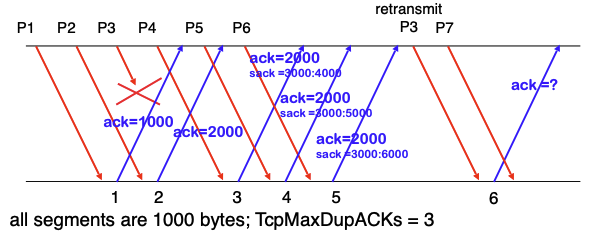
\includegraphics[width=0.8\textwidth]{images/fast-retransmit}
    \label{fig:LABEL}
\end{figure}

\begin{tcolorbox}[
  colback=gray!15,     % background color
  colframe=black!50,    % border color
  boxrule=1pt,       % border thickness
  arc=3mm,             % rounded corners
  left=4mm, right=4mm, top=2mm, bottom=2mm % padding
]
\textbf{When does Fast Retransmit fail to detect loss via duplicate ACKs?}

\vspace{0.3cm}

A. Almost never, it is quasi-optimal \\
B. It fails to detect the loss extremely rarely, but it may often take a long time to detect. \\
C. When one of the last segments of an application layer block is lost, fast retransmit does not detect it. \\
D. It may often fail due to packet re-ordering \\ 
E. I don't know  \\

\textbf{Answer}: C (and probably D). 
\end{tcolorbox}

Most losses are detect via Fast Retransmit (duplicate ACKs), but \textit{\textcolor{red}{few go undetected:}}
\begin{itemize}
	\item Losses are not detect, if (forward or reverse) channel is broken
	\item Isolated/single segments, that are lost, are not detected
	\item Last/trailing segments (of application data), that are lost, may not be detected
		\begin{itemize}
			\item \textcolor{blue}{\textit{Tail Loss Probe}} avoids the latter issue. 
		\end{itemize}
	\item Of course, undetected losses will be eventually detected via RTO timer, but this may take a long(er) time
\end{itemize}

Fast Retransmit may be \textit{\textcolor{red}{inefficient}} if packets are just \textit{\textcolor{red}{reordered}}
\begin{itemize}
	\item The sender retransmits packets that weren't lost - they were just reordered 
	\item 2 counter measures:
		\begin{itemize}
			\item $[$at network layer$]$: \textit{\textcolor{blue}{per-flow load balancing}} avoids sending packets of the same TCP connection over different paths
			\item $[$at transport layer $]$: instead of duplicate ACK, use \textit{\textcolor{blue}{RACK (Recent ACK)}}, which bases retransmissions on \textit{\textcolor{blue}{time}}, not sequence numbers:
				\begin{itemize}
					\item $[$Alg.:$]$: Determine that packet \textit{p} is lost, if:
						\begin{itemize}
							\item Another out-of-order packet is ack'ed and
							\item \textit{p} has not been ack'ed after time = the latest RTT measurement + a configurable "reordering (time) window"
						\end{itemize}
				\end{itemize}

		\end{itemize}

\end{itemize}

\begin{tcolorbox}[
  colback=gray!15,     % background color
  colframe=black!50,    % border color
  boxrule=1pt,       % border thickness
  arc=3mm,             % rounded corners
  left=4mm, right=4mm, top=2mm, bottom=2mm % padding
]
\textbf{If ACK (3) is lost during connection setup, server will:} \\
\begin{enumerate}
	\item retransmit SYN-ACK
	\item keep state information until a timeout occurs
\end{enumerate}

% Quick centered image
\begin{figure}[H]
    \centering
    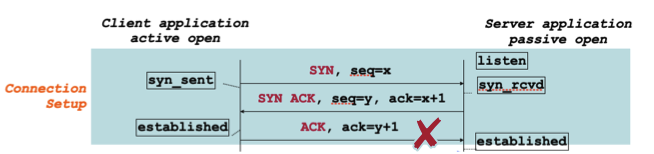
\includegraphics[width=0.8\textwidth]{images/tcp-question-2}
    \label{fig:LABEL}
\end{figure}
\vspace{0.3cm}

A. 1 \\
B. 2 \\
C. 1 and 2 \\
D. None \\
E. I don't now \\ 

\textbf{Answer}: C. \\
When the server receives a SYN packet, it sends the SYN-ACK and enters a \textbf{SYN-received state}, where it keeps all necessary state information about the connection (e.g. IP address and port of the client, the seq number, etc) and does all the usual stuff to detect whether the SYN-ACK is lost. Note that the SYN-ACK does not contain any data in the payload, but it is treated as a normal segment (this is why ACK(3) is y+1 and not y). \\

Thus, if the SYN-ACK and/or ACK(3) are lost, server will retransmit the SYN-ACK. And if there is still no ACK(3) received after retransmission, the server will retransmit again and again until another timer (indicating that the client is not responding) expires. \\

In the first TCP implementations, once TCP entered the SYN-received state, it would stay there for several seconds believing that the SYNACK was lost and retransmitting. \\

\textbf{But this opened the window to a new type of attack!}
\end{tcolorbox}

\section*{Syn flooding attack}
% Quick centered image
\begin{figure}[H]
    \centering
    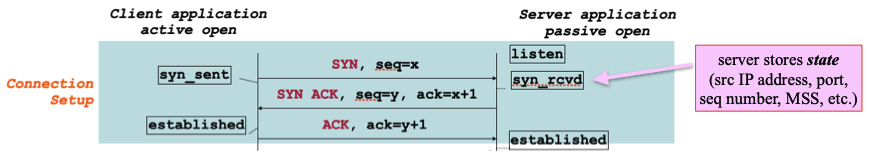
\includegraphics[width=1\textwidth]{images/syn-flooding-attack}
    \label{fig:LABEL}
\end{figure}

\begin{itemize}
	\item Server receives lots of bogus SYN packets from (spoofed) source addresses
	\item Keeps state in kernel $\rightarrow$ runs out of memory $\rightarrow$ legitimate SYN packets are dropped
\end{itemize}

\begin{center}
\textcolor{red}{$\rightarrow$ Denial of Service!}
\end{center}

\textbf{Solution}: \textcolor{blue}{SYN cookie} encodes state in SEQ of SYN ACK

\begin{itemize}
	\item Upon receiving a SYN packet, server keeps \textit{\textcolor{red}{no state}} and sends a special SEQ number = cookie.
	\item Legitimate client sends ACK; server verifies the hash and creates a socket with MSS from cookie
	\item Bogus client sends no ACK; server has lost some time to compute hash, but reserved no memory
\end{itemize}

\begin{center}
\textcolor{red}{$\rightarrow$ SYN flooding is mitigated}
\end{center}

\section*{What if server uses SYN cookies and ACK (3) is lost?}
% Quick centered image
\begin{figure}[H]
    \centering
    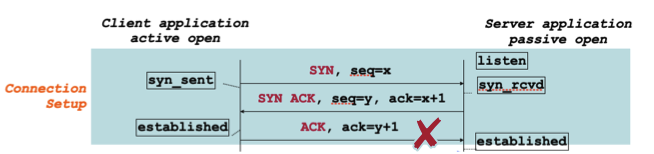
\includegraphics[width=0.8\textwidth]{images/tcp-question-2}
    \label{fig:LABEL}
\end{figure}

\begin{itemize}
	\item If client app sends data with ACK (3), next segment servers as an ACK
		\begin{itemize}
			\item server sees it, validates the cookie, and establish state
		\end{itemize}
	\item If client apps sends no data with ACK (3), we risk a \textcolor{red}{\textit{deadlock}}
		\begin{itemize}
			\item server receives no ACK $\rightarrow$ creates no socket
			\item ACK (3) is never acknowledged, hence never retransmitted
			\item $\rightarrow$ client hangs on established state
			\item $\rightarrow$ such apps (e.g., SSH or mySQL) implement a timeout at the application layer to avoid this
		\end{itemize}
\end{itemize}

\begin{tcolorbox}[
  colback=gray!15,     % background color
  colframe=black!50,    % border color
  boxrule=1pt,       % border thickness
  arc=3mm,             % rounded corners
  left=4mm, right=4mm, top=2mm, bottom=2mm % padding
]
\textbf{With SYN cookies, the response time of SYN-ACK is...}

\vspace{0.3cm}

A. Larger than without SYN cookies \\
B. Smaller than without SYN cookies \\
C. The same \\
D. I don't know \\

\textbf{Answer}: A. Cryptographic calculations take time... Hence, damage from SYN flooding is reduced to \textcolor{blue}{\textit{increased computation time}}, but memory exhaustion is avoided
\end{tcolorbox}
\end{document}	
